% !TeX root=main.tex
\pagenumbering{arabic}
\chapter{مقدمه}
\thispagestyle{empty}
امروزه شبکە‌های اجتماعی یکی از اجزا اصلی تعامل اجتماعی افراد را تشکیل می‌دهد. شبکه‌‌های اجتماعی ابزار قدرت‌مندی برای بیان نظرات و دیدگاە‌های افراد در رابطه با موضوعات متفاوت می‌ باشد. این بستر برای افراد این امکان را فراهم می‌کند که آزادانه نظرات خود را بیان کنند و بازخورد فوری دریافت کنند. همچنین دیدگاه سایر افراد در رابطه با موضوع بیان شده را در این بستر می‌توان مورد بررسی قرار داد.


وابستگی افراد به استفاده از شبکه‌‌های اجتماعی این امکان را فراهم می‌کند تا دادە‌های جمع آوری شده از شبکه‌های اجتماعی را به عنوان منبع مهم برای مطالعه جنبە‌های مختلف موضع‌گیری افراد در زمینە‌های سیاسی و اجتماعی مورد استفاده قرار دهیم.


استخراج خودکار اطلاعات از متون زبان طبیعی از مهم‌ترین زمینە‌های تحقیقاتی می‌باشد. در این راستا می‌توان مسئله تشخیص موضع
\LTRfootnote{\lr{Stance Detection}}
 را تعریف کرد. تشخیص موضع به معنای بیان و تشخیص دیدگاه نویسندە‌ی متن نسبت به یگ گزاره‌ی (موضوع) معین است.

تشخیص موضع در مطالعات تحلیلی برای تشخیص جهت گیری افکار عمومی در رسانە‌های اجتماعی، مانند مسائل سیاسی و اجتماعی، نقش کلیدی ایفا می‌کند. از این رو می‌تواند در شبکە‌های اجتماعی در بستراهداف مختلفی از جمله تصمیمات دولت، تبلیغات، اقناع افکار عمومی مورد استفاده قرار بگیرد. به عبارت دیگر نتایج به دست آمده منجر به دید وسیع‌تری به نظرات عمومی و اخذ تصمیمات بهتر می‌شود.
\section{تعریف مسئله تشخیص موضع}
موضع‌گیری
\LTRfootnote{\lr{Stance}}
به بیان دیدگاه و نظرات افراد راجع به یک گزارە‌ی (موضوع) معین گفته می‌شود
\cite{hardalov-etal-2022-survey}.
تشخیص موضع
\LTRfootnote{\lr{Stance Detection}}
نقشی اساسی در شناخت جهت گیری عمومی در رابطه با مسائل اجتماعی و سیاسی، انتخابات و
موضع تصمیمات دولت ایفا می‌کند
\cite{ALDAYEL2021102597, 10.1145/3209542.3209549}.


مسئله تشخیص موضع در شبکه‌های اجتماعی به این صورت تعریف می‌شود که یک متن نوشته شده
در شبکه اجتماعی (توییت، نظرات و ادعا) و یک موضوع یا هدف مشخص
\LTRfootnote{\lr{Target}}
(شخص، سازمان، جنبش،سیاست) به عنوان ورودی در نظر گرفته می‌شود. هدف تشخیص خودکار موضع متن داده شده نسبت به موضوع مشخص شده است
\cite{ALDAYEL2021102597}.
این یک مسئله به صورت ردە‌بندی است و خروجی یکی از موارد زیر می‌تواند باشد
\cite{li-caragea-2019-multi}.
\begin{enumerate}
	\setlength\itemsep{-0.4em}
	\item موافق
	\LTRfootnote{\lr{Favor/Support}}:
	متن مورد نظر، موضوع تعیین شده را بدون هیچ گونه ابهام تایید می‌کند.
	\item مخالف
	\LTRfootnote{\lr{Against/Oppose}}:
	متن مورد نظر، موضوع تعیین شده را بدون هیچ گونه ابهام رد می‌کند.
	\item بدون نظر
	\LTRfootnote{\lr{None/Neither/Neutral}}:
	متن و موضوع به هم مرتبط نیستند و یا متن به صورت صریح موضوع را رد یا تایید نمی‌کند.
	
\end{enumerate}

\begin{figure}[H]
	\center{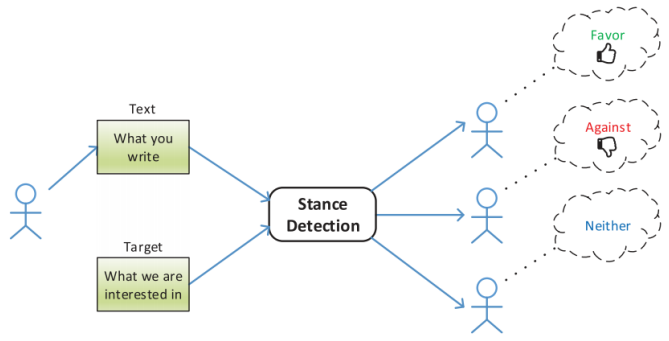
\includegraphics[width=0.6\linewidth]{images/stance_detection.PNG}}
	\caption[تشخیص موضع در شبکه‌های اجتماعی]{تشخیص موضع در شبکه‌های اجتماعی
	\cite{10.1145/3369026}}
\end{figure}

\iffalse
\subsection{کاربردهای تشخیص موضع}
بعد از مطرح شدن تعاریف مختلف مسئله تشخیص موضع، حال به بررسی تعدادی از کاربردهای مطرح شده می‌پردازیم. در مسئله تشخیص موضع، نظر و موضع افراد نسبت به هدف یا موضوع خاص سنجیده می‌شود. با توجه به این تعریف کابردهای زیر مطرح می‌شود.
\begin{enumerate}
	\item 
	 نظرسنجی و بررسی افکار عمومی: مطالعات تشخیص موضع معمولا بر روی محتوا آنلاین انجام می‌شود که موضوع آن مشخص است. از این رو با استفاده از تشخیص موضع خودکار، موافقت یا مخالف عموم افراد جامعه نسبت به موضوع خاصی را می‌توان ارزیابی کرد. این روش می‌تواند جایگزین نظرسنجی‌های سنتی باشد.
	 
	 \item 
	  سیستم‌های توصیە‌گر: در صورتی که موضع افراد نسبت به هدف و موضوعی معین را بدانیم، توصیه کردن محصولات به سادیگی میسر می‌شود.
	 \item 
	 
	 تبلیغات هدفمند: آگاهی از موضع کابران باعث می‌شود تبلیغات به صورت موثر و هدفمند انجام شود.

	 \item
	 
	 تشخیص اخبار جعلی 
	 \cite{popat-etal-2018-declare}
	 و تشخیص شایعه نیز از دیگر کابردهای قابل تعریف به کمک مسئله تشخیص موضع می‌باشند. در این مسائل معمولا از تشخیص موضع ادعا محور استفاده می‌شود.
	 				
\end{enumerate}
\fi
\section{ساختار پایان‌نامه}
این پایان‌نامه در هفت فصل تنظیم شده است. فصل اول مقدمه‌ای از حوزه تحقیقات را شرح می‌دهد. در فصل دوم تعریف مسئله تشخیص موضع به صورت دقیق بیان می‌شود. همچنین جایگاه تشخیص موضع در مقایسه با سایر مسائل مشابه به طور دقیق مشخص می‌شود. فصل سوم به توضیح تعاریف و مفاهیم ابتدایی مورد نیاز برای فهم تشخیص موضع و روش‌های حل مسئله می‌پردازد.
فصل چهارم شامل مروری بر کارهای مرتبط به تشخیص موضع می‌باشد. در فصل پنجم رویکرد حل تشخیص موضع با نظارت شرح داده شده و بررسی می‌شود. فصل ششم نیز شامل معرفی رویکرد پیشنهادی برای تشخیص موضع بدون داده آموزشی می‌باشد. در نهایت در فصل هفتم (فصل آخر) جمع‌بندی از روش‌های حل مسئله انجام شده و پیشنهادهایی برای کارهای آینده ارائه می‌شود.





